\documentclass[12pt,a4paper,parskip=full]{scrartcl}

\usepackage[T2A]{fontenc}
\usepackage[utf8]{inputenc}
\usepackage[russian]{babel}

\usepackage{csquotes}

\usepackage{hyphenat}
\hyphenation{ма-те-ма-ти-ка вос-ста-нав-ли-вать уп-рав-лен-чес-ко-ис-пол-ни-тель-ной}


\usepackage{bbding}
\usepackage{pifont}
\usepackage{wasysym}
\usepackage[margin=1in]{geometry}
\geometry{letterpaper}
\usepackage{xcolor}
\definecolor{red}{HTML}{cc0000}
\definecolor{gray}{HTML}{666666}
\usepackage{sectsty}
\sectionfont{\color{red}}
\subsectionfont{\color{red}}
\subsubsectionfont{\color{red}}
\usepackage{graphicx}
\usepackage{hyperref}
\usepackage{amssymb}
\usepackage[style=footnote-dw]{biblatex}
\bibliography{S@SGuideBib}
\setlength\bibitemsep{0.5\baselineskip}

\usepackage{enumitem}
\setitemize{noitemsep}
% \setlist{noitemsep, topsep=-5pt}
% \setlength\itemsep{-0.10em}

\renewcommand{\labelitemi}{$\cdot$}
\renewcommand{\labelitemii}{$\cdot$}
\makeatletter
\let\latexl@section\l@section
\def\l@section#1#2{\begingroup\let\numberline\@gobble\latexl@section{#1}{#2}\endgroup}
\makeatother

\usepackage[T1]{fontenc}
\fontfamily{verdana}

\usepackage{scrlayer-scrpage}{}
\makeatletter
\renewcommand{\@seccntformat}[1]{}
\makeatother

\setlength\parindent{0pt}{}

\title{\Huge{\color{red}\textbf{ Scrum@Scale 
\textsuperscript{\copyright} 
Руководство}}}
\subtitle{\color{gray}Наиболее полное руководство по Scrum@Scale:\\ Масштабирование, которое работает}
% \author{}
\date{}

\begin{document}

%\tableofcontents
%\newpage

\section{Цель Руководства по Scrum@Scale}

Скрам, как поясняется в Руководстве по Скраму, является фреймворком для разработки, поставки и поддержки сложных продуктов одной командой. С начала существования использование Скрама расширилось для разработки продуктов, процессов, услуг и систем, требующих усилий нескольких команд. Scrum@Scale был создан для эффективной координации этой новой экосистемы команд благодаря оптимизации общей стратегии организации. Эта цель достигается путем создания «минимально жизнеспособной бюрократии» с использованием свободной для масштабирования архитектуры, которая расширяется благодаря обычной Скрам-команде, функционирующей в рамках целой организации.
 
Это Руководство содержит определения компонентов, которые составляют фреймворк Scrum@Scale, включая масштабированные роли, масштабированные события, артефакты организации, а также правила, которые объединяют их вместе.
 
Джефф Сазерленд разработал Scrum@Scale на основе фундаментальных принципов Скрама, сложной адаптационной теории, теории игр и объектно-ориентированной технологии. Это Руководство было создано при участии многих опытных практиков Скрама с учетом результатов их полевых исследований. Цель данного Руководства – предоставить читателю возможность самостоятельно внедрять Scrum@Scale.

\subsection{Почему Scrum@Scale?}

Скрам был разработан для одной команды, чтобы иметь возможность работать c оптимальной производительностью, сохраняя устойчивый темп развития. На практике было обнаружено, что при увеличении количества Скрам-команд в организации производительность (рабочий продукт) и скорость этих команд начинают падать (из-за кросс-командных зависимостей и дублирования работы). Благодаря этому стало очевидно, что для эффективной координации между командами требуется фреймворк, который позволит достичь линейного масштабирования.
 
При использовании свободно масштабируемой архитектуры организация не ограничена в определенном росте комплектом арбитральных правил; скорее она может расти естественным образом, основываясь на своих уникальных потребностях и устойчивом темпе изменений, который может быть принят группами людей, составляющими организацию. Простота модели Scrum@Scale необходима для свободно масштабируемой архитектуры, в которой тщательно избегают усложнений, чтобы не вызывать снижения производительности команд по мере увеличения их количества.
 
Scrum@Scale предназначен для масштабирования организации в целом: всех отделов, продуктов и услуг. Он может быть применен во многих областях во всех типах организаций: в промышленности, правительстве, образовании.


\subsection{Определение Scrum@Scale}

\textbf{Скрам}: фреймворк, в рамках которого люди могут решать сложные, изменяющиеся в процессе работы проблемы, продуктивно и творчески поставлять продукты наивысшей возможной ценности.

Руководство по Скраму представляет собой минимальный набор функций,  позволяющий инспектировать и адаптировать с помощью радикальной прозрачности, чтобы стимулировать инновации, удовлетворенность клиента, производительность и удовлетворение команды. 


\textbf{Scrum@Scale}: фреймворк, в рамках которого сети Скрам-команд, постоянно работающие согласно Руководству по Скраму, могут решать сложные адаптивные проблемы, творчески поставлять продукты наивысшей возможной ценности.

\textbf{ПРИМЕЧАНИЕ}: Этими «продуктами» могут быть аппаратура, программное обеспечение, сложные интегрированные системы, процессы либо сервисы и т.д. в зависимости от того, в какой сфере работают Скрам-команды.

Scrum@Scale:
\begin{itemize}
	\item компактный – минимальный уровень бюрократии;
	\item простой для понимания – состоит только из Скрам-команд;
	\item трудный для совершенного овладения – нуждается во внедрении новой рабочей модели.
\end{itemize}

Scrum@Scale – это фреймворк для масштабирования Скрама, который значительно упрощает его масштабирование, используя сам Скрам.

В Скраме уделено внимание разделению ответственности между «Что» и «Как». То же самое относится и к Scrum@Scale, таким образом сфера полномочий и ответственности четко понятна и позволяет ограничить ненужные организационные конфликты, которые мешают командам в достижении их оптимальной производительности.

Scrum@Scale составлен из компонентов, которые позволяют организации настраивать стратегию их трансформации и применения. Это дает возможность определить цели для инкрементальной приоритизации усилий по изменению в той области, которая считается наиболее ценной или наиболее нуждающейся в изменениях, а затем переходить к другим.

Для  разделения этих двух полномочий Scrum@Scale состоит из двух циклов: Цикла Скрам-Мастера («Как») и Цикла Владельца Продукта («Что»), которые соприкасаются в двух точках. Вместе эти циклы создают мощный фреймворк для координации усилий многих команд в одном направлении.


\subsection{Ценностно-ориентированная культура}

Кроме разделения ответственности между «Что» и «Как», Scrum@Scale нацелен на построение здоровых организаций, создавая ценностно-ориентированную культуру эмпирическим путем. Ценностями Скрама являются: Открытость, Смелость, Сфокусированность, Уважение и Преданность. Эти ценности ведут к эмпирическому принятию решений, которые основаны на «трех китах»: прозрачности, инспекции и адаптации.

Открытость содействует прозрачности в работе и процессах, без которой не будет возможности честно проводить инспекцию и пробовать адаптировать работу и процессы для улучшения. Под Смелостью подразумевается совершение смелых рывков, необходимых для более быстрой поставки ценностей инновационными способами.

Сфокусированность и Преданность отражает то, как мы справляемся с нашими рабочими обязанностями, считая поставку ценности клиенту наивысшим приоритетом. Наконец, все это должно происходить в окружении, основанном на Уважении к людям, выполняющим работу, без которых ничего не может быть создано.

Scrum@Scale помогает организациям процветать, поддерживая трансформационную модель лидерства, которая создает благоприятную среду для работы в устойчивом темпе и ставит на первый план усилия по поставке ценности для клиентов.


\subsection{Составляющие фреймворка Scrum@Scale\textregistered }

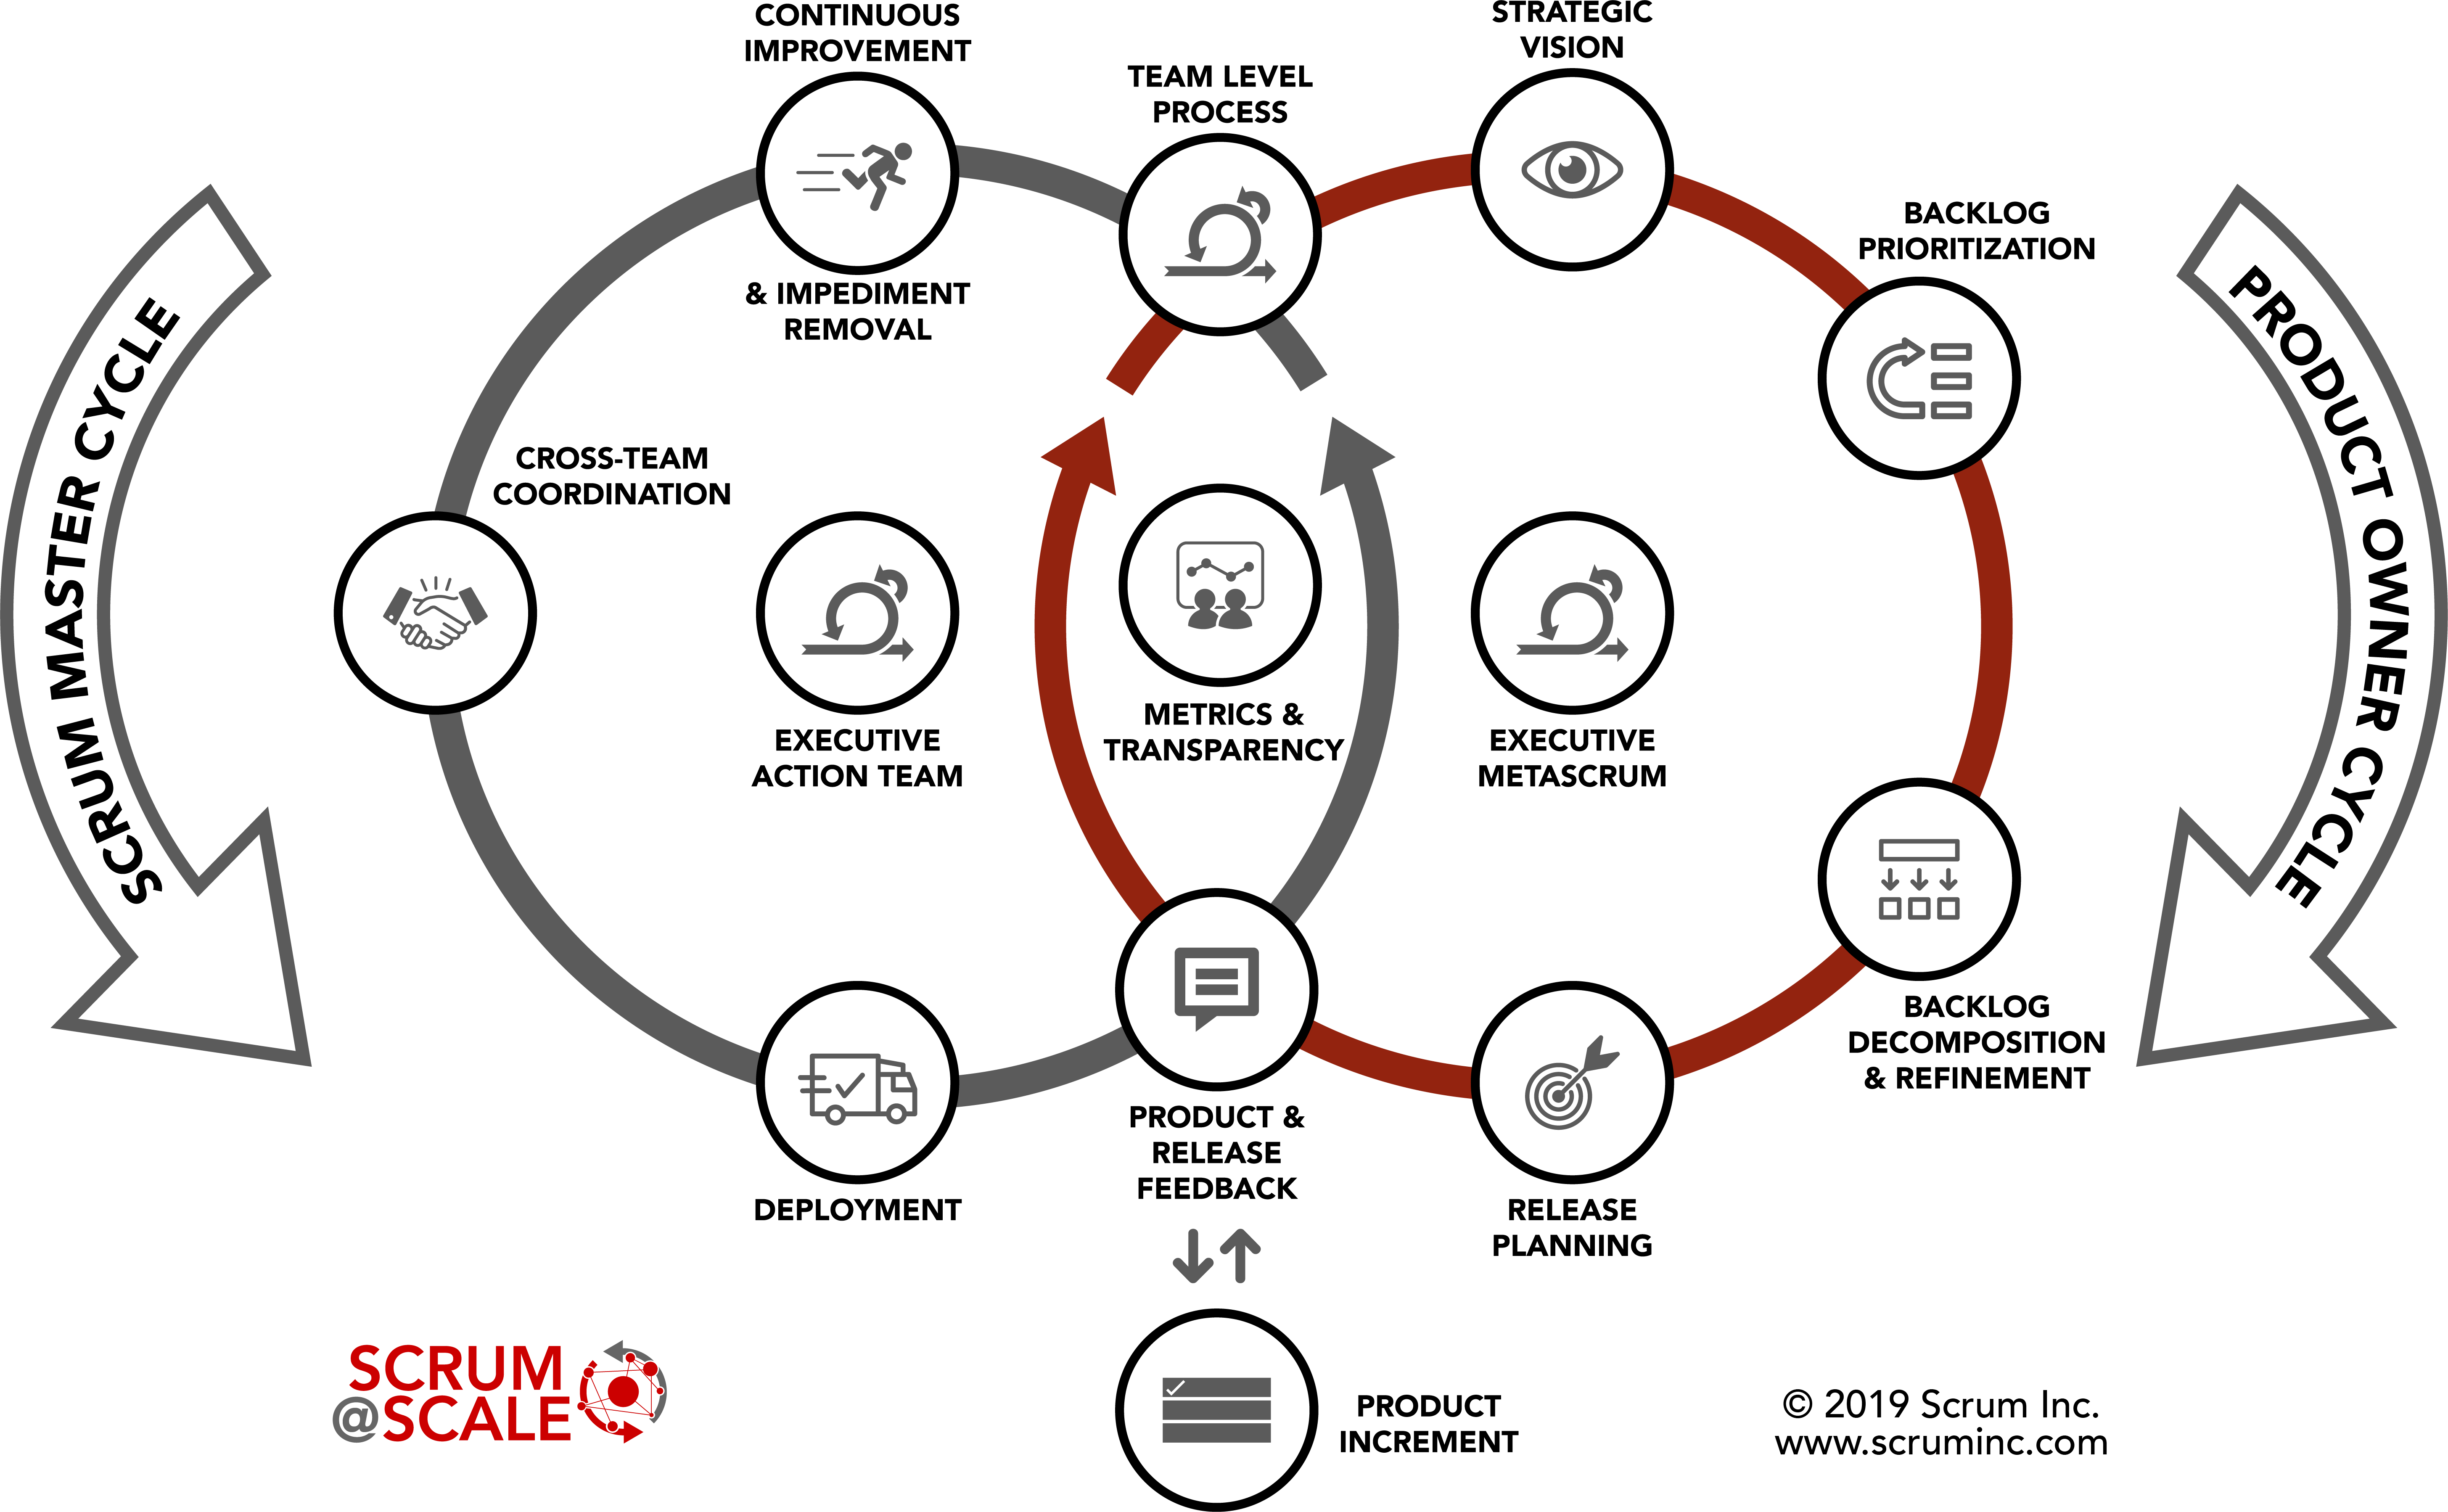
\includegraphics[width=1.0\linewidth]{SMPO-Cycle.png}



\section{Масштабируемая Структура: the Scrum of Scrums}


Набор команд, который необходимо координировать для поставки ценности клиентам, составляет команду  \textbf{Scrum of Scrums (SoS)}. Эта команда сама является Скрам-командой, она ответственна за полностью интегрированный набор потенциально готовых к поставке Инкрементов Продукта в конце каждого Спринта от всех команд.       SoS функционирует как Команда Выпуска, она должна быть в состоянии напрямую доставлять ценность клиентам.

Scrum of Scrums являестя обычной Скрам-командой с обычными ролями, событиями и артефактами, обозначенными в Руководстве по Скраму. Тем не менее, принимая во внимание масштабируемую структуру Scrum@Scale, имеются некоторые изменения.

\subsection{Роли SoS}

SoS должен владеть всеми навыками, необходимыми для поставки полностью интегрированного и готового Инкремента Продукта в конце каждого Спринта и облегчения координации между командной в случае необходимости. (Могут потребоваться опытные архитекторы, QA лидеры, участники Команды Владельцев Продукта и другие наборы навыков.)  

\subsubsection{Команда Владельцев Продукта}

Команда Владельцев Продукта, которая координирует общий Бэклог, насыщающий сеть команд, предствляет собой Скрам-команду, называющуюся \textbf{Командой Владельцев Продукта (Product Owner Team)}. Для каждого SoS имеется Команда Владельцев Продукта, которая выстраивает приоритеты для команд в соответсвии с единым направлением, благодаря чему они могут координировать Бэклоги команд и выстраивать договоренности с Заинтересованными Лицами, для того чтобы поддерживать Бэклог.

Владелец Продукта команды является ответственным за создание и приоритизацию Бэклога команды, он может брать элементы из общего Бэклога SoS для своей команды или создавать независимые элементы по своему усмотрению.

Ключевые функции Команды Владельцев Продукта следующие: 

\begin{itemize}
	\item создать общее видение продукта, сделать его видимым для организации;
	\item обеспечить согласованность с ключевыми Заинтересованными Лицами для обеспечения и поддержки реализации Бэклога;
	\item создать единый, приоритизированный Бэклог; убедиться в отсутствии дублирования работы; 
	\item обеспечить должным образом приоритизацию препятствий и технического долга  в Бэклоге; 
	\item создать минимально единообразный «Критерий Готовности», который применим ко всем командам; 
	\item разрешить зависимости между командами;
	\item создать общий План Выпуска и прогнозировать, опираясь на настоящий План Выпуска (часто называемый Техническая дорожная карта);
	\item выбирать и отслеживать показатели, которые дают представление о продукте и рынке.
\end{itemize}

Команды Владельцев Продукта, как и команды SoS, функционируют сами как Скрам-команды. Это значит, что они должны иметь Скрам-Мастера, который поддерживает команду в дискуссиях. Им также нужен один человек, отвечающий за создание единого Бэклога Продукта для всех команд, объединенных в Scrum of Scrums. Этот человек  назначается  \textbf{Главным Владельцем Продукта (Chief Product Owner).}

\subsubsection{Главный Владелец Продукта (The Chief Product Owner, CPO)}

 \textbf{Главный Владелец Продукта} (CPO) координирует приоритеты среди Владельцев Продукта, которые работают с отдельными командами. Они выстраивают приоритеты в Бэклоге в соответствии с потребностями Заинтересованных Лиц и Клиентов. Это может быть Владелец Продукта одной из команд либо другой человек, назначенный на эту роль. Обязанности Главного Владельца Продукта такие же, как и у обычных Владельцев Продукта, только масштабируемые:

\begin{itemize}
	\item определение стратегического видения для SoS; 
	\item создание единого приоритизированного  Бэклога ценностей для поставки всем командам;
	\begin{itemize}
		\item ПРИМЕЧАНИЕ: Обычно это большие Элементы Бэклога Продукта, которые Уточняются и Декомпозируются Владельцами Продуктов на уровне команд.
	\end{itemize}
	\item работа в тесном контакте с SoSM (описание ниже) над созданием Плана Выпуска для реализации эффективного развертывания через Команду Владельцев Продукта; 
	\item мониторинг отзывов клиента относительно продукта и корректировка Бэклога в соответствии с ними; 
	\item на Управленческом/МетаУровне – возглавление МетаСкрама, где презентуется Бэклог Продукта и достигаются договоренности с Заинтересованными Лицами. 
\end{itemize}



\subsubsection{Scrum of Scrums Master (SoSM)}

Скрам-Мастер для Scrum of Scrums называется \textbf{Scrum of Scrums Master (SoSM)}. SoSM отвечает за выпуск усилий объединенных команд и обязан: 

\begin{itemize}
	\item сделать прогресс видимым;
	\item сделать Бэклог препятствий видимым для организации; 
	\item устранять препятствия, которые команды не смогут решить сами; 
	\item содействовать приоритизации проблем, уделяя особое внимание зависимостям между командами; 
	\item улучшать эффективность Scrum of Scrums;
	\item тесно сотрудничать с Владельцами Продукта, чтобы развернуть потенциально готовый к выпуску Инкремент Продукта в конце каждого Спринта;
	\item координировать развертывание команд с планами выпусков Владельца Продукта. 
	
\end{itemize}

\subsection{События SoS}

\subsubsection{Работа с препятствиями на уровне SoS}

SoSM должен способствовать такому событию, как Бэклог Уточнения (Backlog Refinement), при котором препятствия идентифицируются как «готовые» для удаления, и команда определяет, как лучше их удалить и как узнать, что они уже «закончены». Этот Бэклог удаления препятствий приоритизируется для команд на том же  уровне, что и SoS CPO \& Команда Владельцев Продукта.

Особое внимание следует уделить Ретроспективе  SoS (SoS Retrospective), когда представители команд делятся новыми знаниями или улучшениями процессов, в которых их команды преуспели, для распространения лучших практик среди всех команд в SoS.

\subsubsection{Масштабируемый Ежедневный Скрам (Scaled Daily Scrum, SDS)}

SoS должен реагировать в реальном времени на препятствия, возникающие перед командой, для этого как минимум один участник команды (обычно это Скрам-Мастер каждой команды) должен посещать  \textbf{Масштабируемый Ежедневный Скрам (Scaled Daily Scrum, SDS)}. Любой человек или несколько людей из участвующих команд могут посещать Масштабируемый Ежедневный Скрам при необходимости. Кроме того, Масштабируемый Ежедневный Скрам (SDS):

\begin{itemize}
	\item ограничивается 15 минутами (либо меньше);
	\item нуждается в присутствии представителей каждой из команд, включая Команды Владельцев Продукта; 
	\item является форумом, где представители команд обсуждают, что идет хорошо, что сделано и как команды могут работать более эффективно.
\end{itemize}
	
Несколько примеров дискуссии:
\begin{itemize}
	\item Какие проблемы влияют на мою команду и мешают достижению Цели Спринта (либо влияют на ближайший выпуск)?
	\item Делает ли моя команда что-нибудь, что может негативно повлиять на достижение Цели Спринта другой команды (либо повлиять на ближайший выпуск)?
	\item Увидели ли мы какие-либо новые зависимости между командами либо нашли способ, как мы можем решить существующую зависимость? 
	\item Какие решения проблем мы нашли, могут ли они быть использованы другими командами? 
\end{itemize}

\section{Управленческий уровень/МетаУровень}

\subsection{Управленческо-исполнительная команда (The Executive Action Team)}

Роль Скрам-Мастера, которая является частью Scrum of Scrums для целой организации, называется \textbf{Управленческий МетаСкрам (Executive Action Team (EAT)}. Команда руководителей создает своего рода «гибкий пузырь» (agile bubble) в организации, где Относительная модель работает в соответствии со своими методиками и процедурами, эффективно интегрирующими все части организации, которая не является гибкой. EAT владеет гибкой экосистемой, внедряет ценности Скрама и удостоверяется в том, что роли Скрама созданы и имеют должную поддержку. 

Управленческо-исполнительная команда является финальным пунктом для препятствий, которые не могут быть устранены в SoS. Она должна состоять из людей, наделенных политическими и финансовыми полномочиями для устранения препятствий. Функцией EAT является координация нескольких SoS (либо SoSoS) и взаимодействие с любой негибкой частью организации. Как и любая другая команда, EAT нуждается в своем Владельце Продукта и Скрам-Мастере, которые должны встречаться ежедневно. У них также должен быть свой прозрачный Бэклог. 

Образец диаграммы, который показывает, как EAT координирует 5 групп, состоящих из 25 команд: 

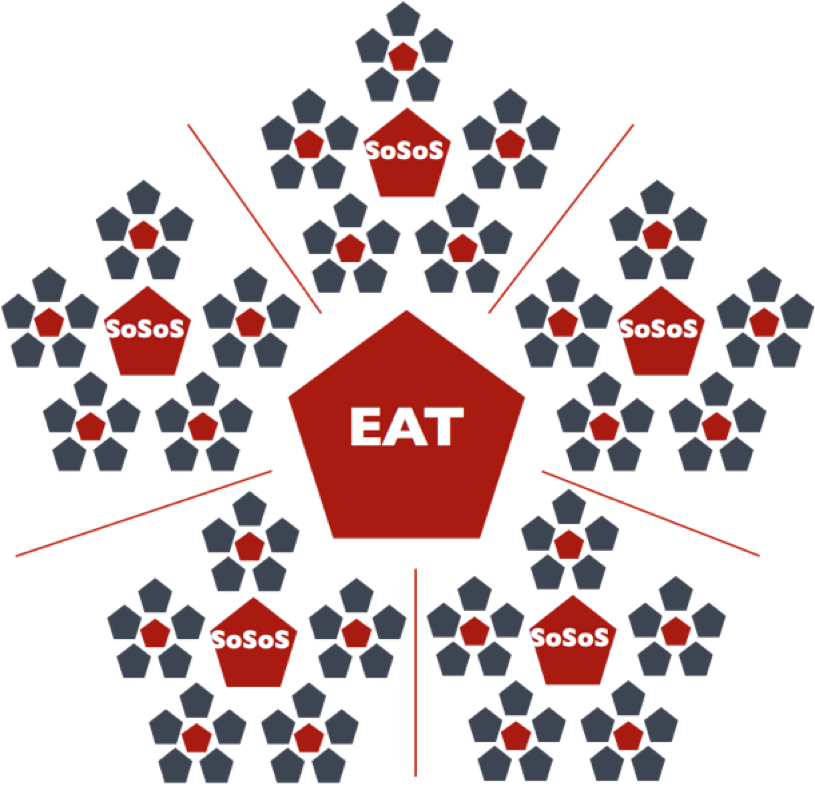
\includegraphics[width=\textwidth,height=\textheight,keepaspectratio]{SoS-EAT.png}

\subsubsection{Бэклог EAT и ее ответственность}

Скрам – это гибкая операционная система, которая значительно отличается от традиционного управления проектами. Вся Скрам-организация отчитывается EAT, отвечающей за внедрение гибкой операционной системы путем основания, поддержки и усовершенствования внедрения Скрама в организации. 

Роль EAT  заключается в создании Бэклога трансформации организации (список заданий, связанных с agile, которые должны быть осуществлены) и слежении за ним. К примеру, если существует традиционный цикл развития продукта в организации старого типа, то необходимо создавать, внедрять и поддерживать новый цикл развития продукта. Он обычно улучшает качество и способствует решению проблем лучше, чем старый метод, но реализуется другим путем с другими правилами и руководствами. EAT способствует созданию организации Владельцев Продукта, поддерживает ее и оказывает должное финансирование, а также презентует эту организацию в EAT. 

EAT отвечает за качество Скрама в организации. Ее обязанности включают следующее (но не ограничиваются только перечисленным): 

\begin{itemize}
	\item создание гибкой операционной системы для формирования Относительной модели по мере ее масштабирования в организации, включая общие корпоративные правила, процедуры и руководства для обеспечения лучшей гибкости; 
	\item измерение и улучшение качества Скрама в организации;
	\item создание условий в организации для гибкости бизнеса; 
	\item формирование центра для постоянного развития специалистов Скрама; 
	\item поддержка и изучение новых возможностей и путей работы. 
\end{itemize}

\subsection{Управленческий МетаСкрам (Executive MetaScrum, EMS)}

Команды Владельцев Продукта позволяют проектировать сети Владельцев Продукта, которые можно бесконечно масштабировать вместе со связанными с ними SoS. Команда Владельцев Продукта для целой организации, которая встречается с ключевыми Заинтересованными Лицами, называется \textbf{Управленческим МетаСкрамом}. Управленческий МетаСкрам владеет видением организации и устанавливает стратегические приоритеты, выстраивает общие цели для команд.

Пример диаграммы, которая демонстрирует, как Управленческий МетаСкрам координирует 5 групп, состоящих из 25 команд: 

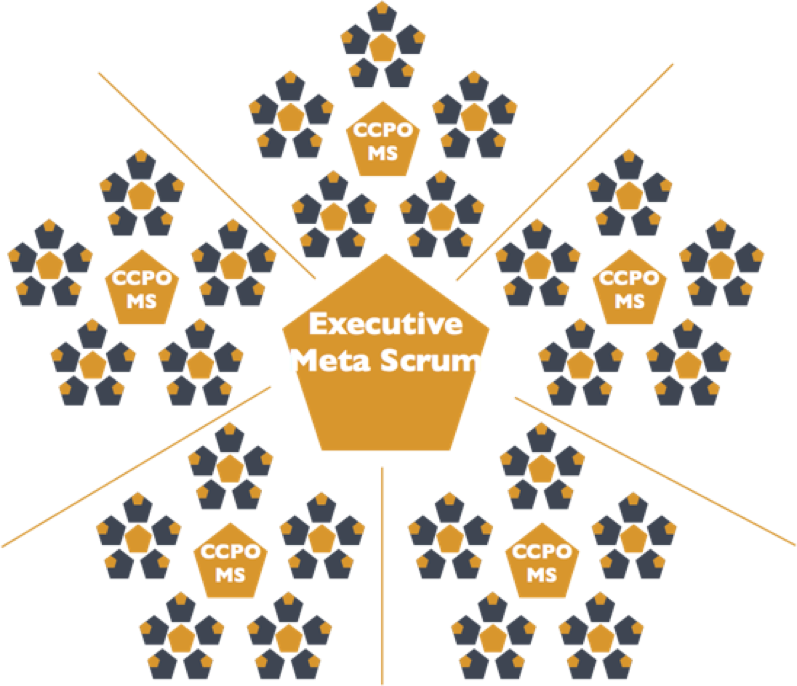
\includegraphics[width=1.0\linewidth]{ExecMetaScrum.png}

Управленческий МетаСкрам достигает согласия с ключевыми Заинтересованными Лицами путем проведения такого события, как \textbf{МетаСкрам (MetaScrum Event)}, которое происходит регулярно как минимум один раз за Спринт.

\begin{itemize}
	\item Участники Управленческого МетаСкрама (либо их заместители) посещают МетаСкрам, где Главный Владелец Продукта презентует Бэклог Продукта Владельцам Бизнеса, контролирующим финансирование, персонал и обязательство перед клиентами. Они адресуют все необходимые изменения в стратегии, финансировании, распределении ресурсов, развертывании и работают с Главными Владельцами Продукта для достижения согласия на Бэклоге Продукта, который они будут поддерживать до следующего МетаСкрама.
	\item Это событие представляет собой форум для Лидеров, Ключевых Заинтересованных Лиц и Владельцев Бизнеса для выражения своих желаний и иногда острых потребностей, которые могут повлиять на реструктуризацию Бэклога Главного Владельца Продукта.
\end{itemize}

\section{Масштабирование}

\subsection{Масштабирование SoS}

В зависимости от размера организации и внедрения для поставки очень сложных продуктов может потребоваться более одного SoS. В этом случае \textbf{Scrum of Scrum of Scrums (SoSoS)} может быть создан из нескольких Scrum of Scrums. SoSoS – пример того, как могут быть бесконечно масштабированы Скрам-команды. У каждого SoS должны быть свой SoSM и масштабируемые версии каждого артефакта и события. 

Масштабирование SoS уменьшает количество путей коммуникации в организации, благодаря чему сложность компенсируется. Таким образом, SoSoS взаимодействует с SoS так же, как и SoS с каждой Скрам-командой, что способствует линейному масштабированию.

Образцы диаграмм:

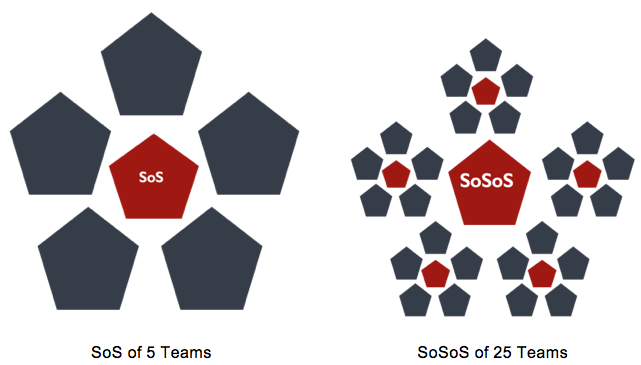
\includegraphics[width=1.0\linewidth]{Sos-R2.png}

\textbf{\textsc{ПРИМЕЧАНИЕ:}} В то время как Руководство по Скраму определяет оптимальный размер команды от 3 до 9 человек, исследования Гарварда показали, что лучшее количество – 4,6 человека. Эксперименты с высокопроизводительными Скрам-командами выявили, что рабочие команды из 4–5 человек наиболее оптимальны. Понятно, что и для линейного масштабирования оптимальное количество людей в команде будет таким же. Поэтому в приведенных выше диаграммах пятиугольники были выбраны для демонстрации команд, состоящих из 5 человек. 
Эти диаграммы даны только в качестве примера, диаграммы Ваших организаций могут сильно отличаться. 


\subsection{Масштабирование Команды Владельцев Продукта}

Подобно тому, как SoS может вырасти в SoSoS, Команда Владельцев Продукта может масштабироваться с использованием этого же механизма. Для таких масштабируемых единиц нет специального названия, также и у Главных Владельцев Продукта нет новых специальных расширенных названий. Мы призываем каждую организацию придумать свои собственные. Для диаграмм, представленных ниже, мы решили добавлять слово «Главный» (Chief) для последующих масштабируемых ролей Владельцев Продукта.

Образцы диаграмм:

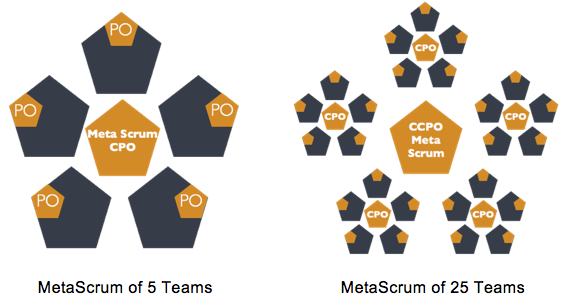
\includegraphics[width=1.0\linewidth]{MetaScrum-R2.png}

\textbf{ПРИМЕЧАНИЕ:} Как указано выше, данные пятиугольники показывают Скрам-команды идеального размера и команды Владельцев Продукта также идеального размера. Эти диаграммы представлены только в качестве примера, диаграммы Вашей организации могут сильно отличаться. 

\section{Цикл Скрам-Мастера – Координация «Как»}

Организация Скрам-Мастеров (SoS, SoSoS и EAT) работает как единое целое для того, чтобы завершить другие составляющие Цикла Скрам-Мастера. Уникальными компонентами для Цикла Скрам-Мастера являются: \textbf{ Постоянное Улучшение, Удаление Препятствий, Кросс-командная Координация и Развертывание.}

\subsection{Постоянное Улучшение и Удаление Препятствий}

Цели Постоянного Улучшения и Удаления Препятствий следующие:

\begin{itemize}
	\item определить проблемы и переосмыслить их как возможности; 
	\item поддержать здоровую и структурированную среду для приоритизации и удаления препятствий, а затем проверки результатов улучшений; 
	\item обеспечить видимость в организации для осуществления изменений.
\end{itemize}

\subsection{Кросс-командная Координация}

Цели для Кросс-командной Координации:

\begin{itemize}
	\item координировать процессы для нескольких связанных между собой команд; 
	\item смягчить межкомандные зависимости, чтобы они не становились препятствиями;
	\item поддерживать согласованность командных норм и руководящих принципов для последовательного результата.
\end{itemize}

\subsection{Развертывание}

Поскольку целью SoS является функционирование в качестве команды-выпуска, развертывание продукта входит в его ответственность, в то время как то, что находится в выпуске, относится к ответственности Владельца Продукта. Цели развертывания:

\begin{itemize}
	\item обеспечить постоянный поток поставки ценного и готового продукта клиентам; 
	\item объединить работу разных команд в один целостный продукт; 
	\item обеспечить высокое качество обслуживания клиентов.
\end{itemize}

\section{Цикл Владельца Продукта  – Координация «Что»}

 Уникальными компонентами цикла Владельца Продукта являются: \textbf{Стратегическое видение, Приоритизация Бэклога, Декомпозиция и Уточнение Бэклога, Планирование Выпуска.}

\subsection{Стратегическое видение}

Цели установления Стратегического видения: 

\begin{itemize}
	\item отчетливо установить общее направление для организации;
	\item точно определить причину существования организации; 
	\item описать, как организация будет использовать свои активы для поддержки миссии;
	\item соответствующе реагировать на быстро изменяющиеся условия рынка. 
\end{itemize}

\subsection{Приоритизация Бэклога}

Цели Приоритизации Бэклога: 

\begin{itemize}
	\item определять четкий порядок поставки продуктов, функций и услуг;  
	\item отражать создание ценности, снижение  рисков  и внутренние зависимости в упорядочении Бэклога;
	\item приоритизировать инициативы высшего уровня для гибкой организации через Уточнение и Декомпозицию Бэклога. 
\end{itemize}

\subsection{Декомпозиция и Уточнение Бэклога}

Цели Уточнения и Декомпозиции Бэклога: 

\begin{itemize}
	\item разделять сложные продукты либо проекты на независимые функциональные части, чтобы они могли быть выполнены в рамках одного Спринта одной командой; 
	\item собирать и анализировать возникающие требования и отзывы клиентов; 
	\item убедиться в том, что все элементы Бэклога на самом деле «готовы», чтобы их можно было взять индивидуальным командам.
\end{itemize}

\subsection{Планирование Выпуска}

Цели Планирования Выпуска: 

\begin{itemize}
	\item прогноз поставки ключевых функций и возможностей; 
	\item сообщение ожидаемых сроков поставки Заинтересованным Лицам; 
	\item обновление приоритизации при необходимости.
\end{itemize}

Обратите внимание, что Планирование Выпуска может объединять один либо несколько Выпусков продукта для клиента. Это планирование более высокого уровня, чем один Спринт, обычно оно охватывает период от одного до шести месяцев.

\section{Соединение Цикла Скрам-Мастера и Владельца Продукта}

Цикл Владельца Продукта и Цикл Скрам-Мастера имеют 2 пункта соприкосновения: \textbf{Уровень Команды и Отзыв Продукта и Выпуска}. Оба цикла нуждаются в \textbf{Показателях и Прозрачности}.

\subsection{Уровень команды}

 \textbf{Уровень команды} является первой точкой соприкосновения между Скрам-Мастером и Владельцем Продукта и четко изложен в Руководстве по Скраму. Он состоит из трех артефактов, пяти событий и трех ролей. Цели на уровне команды:

\begin{itemize}
	\item максимизировать поток выполненной и качественно протестированной работы;
	\item повышать производительность команды на протяжении времени; 
	\item работать устойчиво и с пользой для команды;
	\item ускорить цикл обратной связи с клиентом.
\end{itemize}

\subsection{Отзыв о Продукте и Выпуске}

\textbf{Отзыв о Продукте и Выпуске} является второй точкой соприкосновения цикла Скрам-Мастера и Владельца Продукта. Отзыв о продукте способствует постоянному улучшению путем корректировки Бэклога Продукта, в то время как Отзыв о Выпуске поможет улучшить механизм Развертывания. Цели получения и анализирования Отзыва:

\begin{itemize}
	\item подтвердить предположения;
	\item понять, как клиенты используют продукт и взаимодействуют с ним;
	\item собрать идеи для новых функциональностей и функций;
	\item определить улучшения для существующей функциональности; 
	\item обновить прогресс  в завершении продукта/проекта для уточнения Плана Выпуска и согласования с Заинтересованными Лицами; 
	\item определить улучшения для развертывания методов и механизмов. 
\end{itemize}

\subsection{Показатели и Прозрачность}

Радикальная прозрачность необходима для оптимального функционирования Скрама, но ее можно достичь только в организации, принявшей ценности Скрама. Это дает организации возможность честно оценивать свой прогресс, а также инспектировать и адаптировать свои продукты и процессы. Такой подход является основой эмпирической природы Скрама, изначально изложенной в Руководстве по Скраму.

Оба цикла (Скрам-Мастера и Владельца Продукта) нуждаются в показателях; решение о том, какие показатели использовать, могут быть приняты отдельно организациями Скрам-Мастеров и Владельцев Продукта. Показатели могут быть предназначены как для организации, так и для конкретных функций в этих организациях. Scrum@Scale не вынуждает внедрять какие-либо специальные показатели, но предполагает, что организация как минимум должна измерить:


\begin{itemize}
	\item производительность, например, изменение количества рабочего продукта, доставленного в Спринте;
	\item поставку ценностей, например, ценности бизнеса на единицу усилий команды;
	\item качество, например, частота появления дефектов системы и время упадка системы;
	\item устойчивость, например, удовлетворение команды. 
\end{itemize}

Целями Показателей и Прозрачности являются: 

\begin{itemize}
	\item предоставление всем лицам, принимающим решения, включая членов команды, соответствующего контекста для принятия правильных решений;
	\item максимальное сокращение циклов Отзыва, чтобы избежать чрезмерной коррекции;
	\item достижение минимальных дополнительных усилий со стороны команд, Заинтересованных Лиц и руководства.
\end{itemize}

\section{Руководство по началу работы со Scrum@Scale}

При работе с большим количеством команд критически важно создать масштабируемую  \textbf{Относительную модель (Reference model)} для небольшого количества команд. Любые недочеты во внедрении Скрама начнут возрастать при развертывании нескольких команд. Многие проблемы масштабирования Скрама будут связаны с организационной политикой и процедурами либо с практиками разработки, которые блокируют высокую производительность и мешают реализации планов команд. 

Более того, первая трудность заключается в создании небольшого количества команд, которые хорошо используют Скрам. Этого лучше всего достичь созданием \textbf{Управленческо-исполнительной команды (Executive Action Team, EAT)}, которая ответственна за развитие и реализацию стратегии трансформации. В EAT должны входить люди, наделенные политическими и финансовыми полномочиями, для гарантирования существования Относительной модели. Этот набор команд решает организационные проблемы, блокирующие гибкость, и создает Относительную модель для Скрама, которая, как известно, работает в организации и может использоваться в качестве шаблона для масштабирования Скрама во всей организации.

По мере ускорения работы Относительной модели становятся очевидными препятствия и узкие места, которые задерживают поставку, производят отходы или мешают гибкости. Наиболее эффективный способ устранения этой проблемы – это распространение Скрама по всей организации для оптимизации всего потока создания ценностей.

Scrum@Scale обеспечивает достижение линейного масштабирования производительности благодаря насыщению организации Скрамом и органичному распределению скорости и качества в соответствии со стратегией, продуктом и услугами организации.

\section{Некоторые заметки, касающиеся Конструирования структуры Организации}

Свободная от масштабирования (scale-free) природа Scrum@Scale позволяет конструировать структуру организации, которая будет основана на тех же компонентах, что и сам фреймворк. Это позволяет свободно перебалансировать и изменять команды в зависимости от нужд рынка. По мере роста организации важно использовать преимущества от распределенных команд. Некоторые организации нанимают талантливых людей, в противном случае они могут расширяться и сокращаться по мере необходимости с помощью аутсорсинга. Scrum@Scale демонстрирует, как развиваться и расти, избегая долгого времени поставки продуктов на рынок, скомпрометированных  коммуникаций и низкого качества, обеспечивая линейное масштабирование как по размеру, так и по глобальному распределению. 

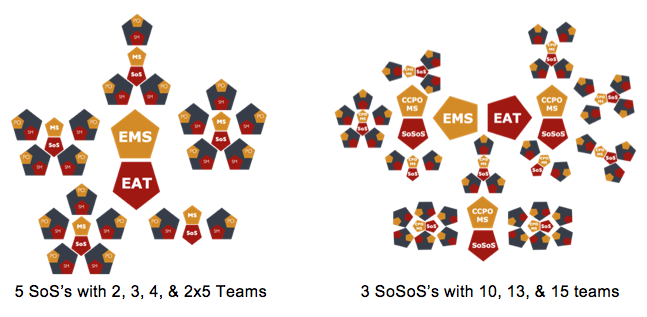
\includegraphics[width=1.0\linewidth]{VariableSoS-R2.png}
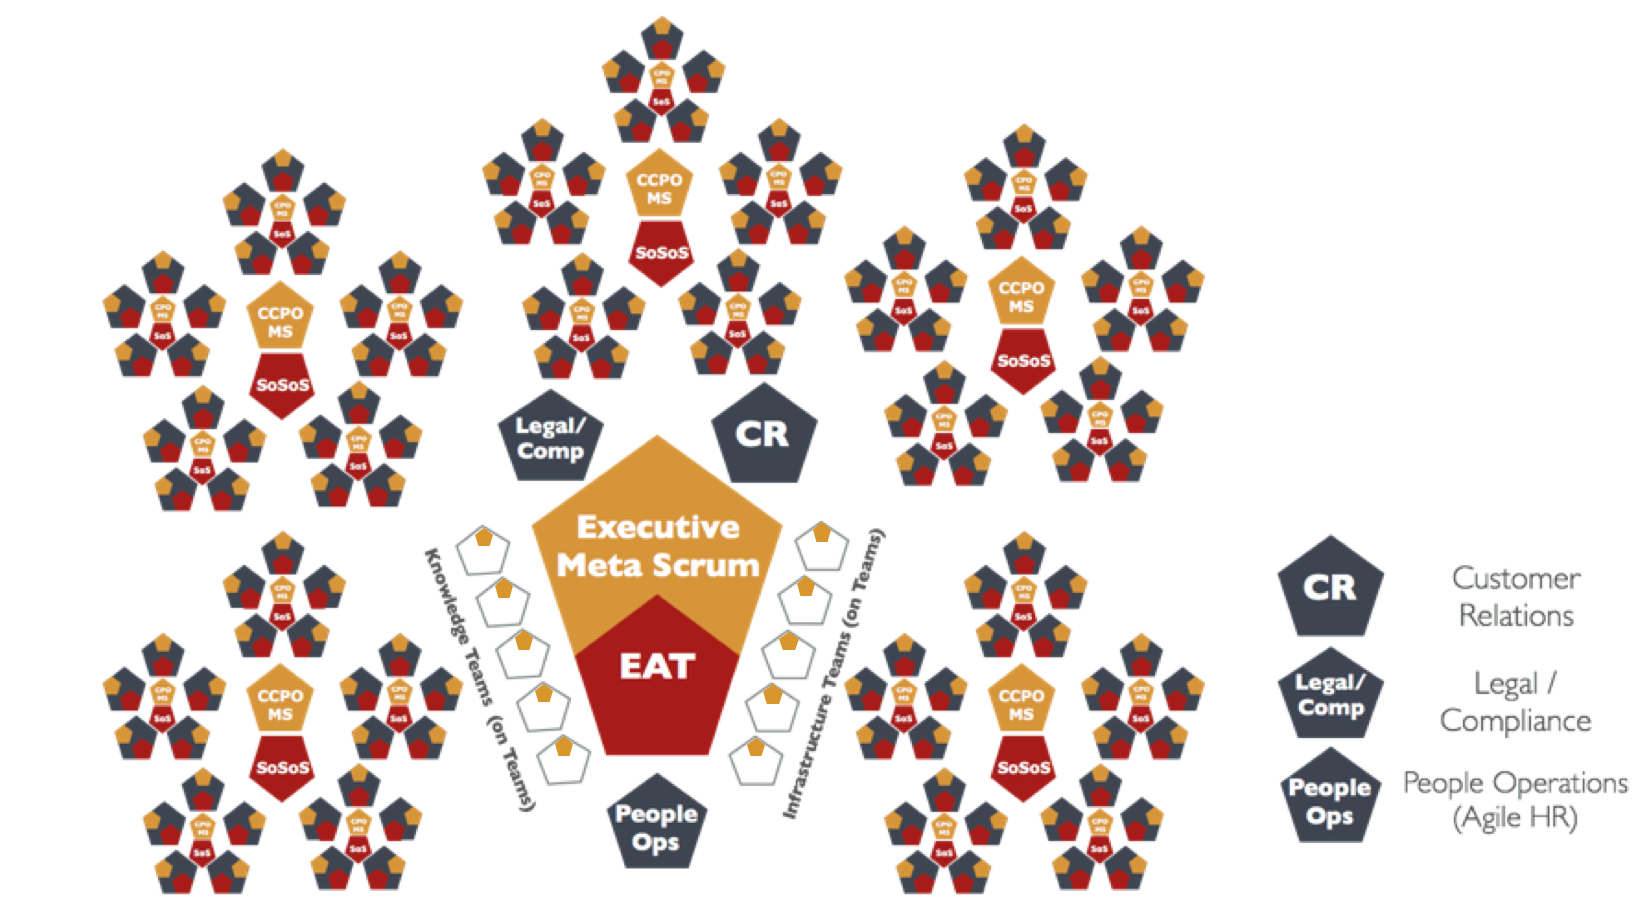
\includegraphics[width=1.0\linewidth]{OrganizationalDiagram.png}

На этой диаграмме  \textbf{Команды Компетенций и Инфраструктуры (Knowledge \& Infrastructure Teams)} представляют виртуальные команды специалистов, которых слишком мало для укомплектования каждой команды. Их координация со Скрам-командами происходит посредством соглашений об уровне обслуживания, где запросы исходят от Владельца Продукта каждой специализации, который позже конвертирует эти требования в прозрачный Бэклог Продукта. Важным примечанием является то, что эти команды НЕ являются отдельными группами людей, которые сидят вместе (именно поэтому они представлены как прозрачные пятиугольники); члены этих команд находятся в Скрам-командах, но они создают свой виртуальный Скрам для расширения Бэклога Продукта и для улучшения процесса. 

\textbf{Отдел Связи с Клиентами, Правовой Отдел/Комплаенс и Отдел Кадров} тоже включены, так как это важные и нужные части организации, они существуют как независимые Скрам-команды, с которыми все другие Скрам-команды могут сотрудничать. 

Последнее примечание относительно EAT и EMS: на этой диаграмме они показаны как перекрывающиеся, поскольку некоторые представители являются частью обеих команд. В очень маленьких организациях EAT и EMS могут состоять из одних и тех же членов команды.

\section{Послесловие}

Scrum@Scale создан для масштабирования производительности, чтобы вся организация обеспечивала поставку удвоенной ценности в два раза быстрее с более высоким качеством и в значительно улучшенной рабочей среде. Большие организации, которые должным образом внедряют этот фреймворк, могут снизить затраты на свои продукты и услуги,  повышая в то же время качество и инновационность. 

Scrum@Scale создан таким образом, чтобы насытить организацию Скрамом. Все команды, работающие в разных отраслях, включая Лидерство, Управление Персоналом, Право, Консалтинг и Тренинг, а также команды по продуктам и услугам, внедряют единый стиль Скрама для оптимизации и усиления организации. 

Хорошо реализованный Скрам может управлять всей организацией. 


\section{Благодарность}

Мы очень признательны IDX за создание Scrum of Scrums, который впервые позволил Скраму масштабироваться для сотен команд. PatientKeeper мы благодарны за создание MetaScrum, который обеспечил быструю доставку инновационных продуктов, а также OpenView Venture Partners – за масштабирование Скрама на всю организацию. Мы ценим вклад со стороны Intel, поскольку более чем 25 000 человек, работающих в Скраме, научили нас «что ничего не масштабируется» кроме свободной для масштабирования архитектуры, а также SAP с самой большой Скрам-командной продуктовой организацией, которая научила нас, что участие Менеджмента в MetaScrum – это ключ для совместной работы 2000 Скрам-команд. 

Аджайл Коучи и Тренеры, которые внедряют эту концепцию в Amazon, GE, 3M, Toyota, Spotify, Maersk, Comcast, AT\&T и многих других организациях, работающих вместе с Джеффом Сазерлендом, очень сильно помогали в тестировании этих концепций в большом количестве компаний из разных отраслей. 

И в конечном итоге мы благодарны Ави Шнайеру, Алексу Сазерленду и Джессике Ларсен за неоценимый вклад в разработку и редактирование этого документа. 

\pagebreak

\printbibliography

\end{document}